\documentclass[aspectratio=169,11pt]{beamer}

\usepackage[utf8]{inputenc}
\usepackage[T1]{fontenc}
\usepackage[serbian]{babel}

\usepackage{amsmath}
\usepackage{amssymb}

\usepackage{tikz}
\usepackage{pgfplots}
\graphicspath{{./presentation/}}

\usetikzlibrary{positioning}
\setbeamertemplate{navigation symbols}{}

\usepackage{ragged2e}
%\usepackage{etoolbox}
%\apptocmd{\frame}{}{\justifying}{}
\setlength{\parskip}{0.2cm}

\usepackage{subfig}
\captionsetup[subfloat]{labelformat=simple}
\renewcommand{\thesubfigure}{\alph{subfigure})}

\usepackage[normalem]{ulem}

% =========================================================
% COLORS
% =========================================================

\definecolor{background}{HTML}{0B0D10}
\definecolor{blueColor}{HTML}{4CC9F0}
\definecolor{grayColor}{HTML}{8A9099}
\definecolor{whiteColor}{HTML}{DCE7EB}
\definecolor{redColorHard}{HTML}{F05A67}
\definecolor{redColorLight}{HTML}{B86A6A}

\newcommand{\blueColor}[1]{\textcolor{blueColor}{#1}}
\newcommand{\grayColor}[1]{\textcolor{grayColor}{#1}}
\newcommand{\whiteColor}[1]{\textcolor{whiteColor}{#1}}
\newcommand{\redColor}[1]{\textcolor{redColorLight}{#1}}

\newcounter{ciljcounter}
\newcommand{\metodologijaCilj}[1]{%
    \stepcounter{ciljcounter}%
    \textcolor{blueColor}{\uline{Cilj \theciljcounter:}} #1%
}

\newcommand{\metodologijaProblem}{\textcolor{redColorHard}{\uline{problem:}}}

% =========================================================
% BEAMER COLORS
% =========================================================

\setbeamercolor{background canvas}{bg=background}
\setbeamercolor{normal text}{fg=whiteColor}
\captionsetup[subfloat]{labelfont={color=whiteColor}}

% =========================================================
% SLIDE HEADER
% =========================================================

\setbeamertemplate{frametitle}{

    \vspace{0.25cm}

    \begin{beamercolorbox}[
        wd=\paperwidth,
        leftskip=0.99cm,
        rightskip=0.65cm]
        {frametitle}
        {\Large\textcolor{blueColor}{\insertframetitle}}
    \end{beamercolorbox}

    \nointerlineskip
    \vspace{0.5cm}

    \textcolor{blueColor}{\rule{2.0cm}{1pt}}

    \vspace{0.25cm}
}

% =========================================================
% FOOTER / SLIDE NUMBER
% =========================================================

\setbeamertemplate{footline}{
    \begin{beamercolorbox}[
        wd=\paperwidth,
        ht=0.45cm,
        dp=0.2cm
    ]{footline}

        \hfill
        {\scriptsize
        \textcolor{grayColor}{
            \insertframenumber
        }}
        \hspace{0.45cm}

    \end{beamercolorbox}
}

% =========================================================
% BACKGROUND NETWORK
% =========================================================

\newcommand{\networkbackground}{

\begin{tikzpicture}[
    remember picture,
    overlay
]

\newcommand{\bcYone}{8cm}
\newcommand{\bcYtwo}{8.5cm}
\newcommand{\bcConnection}{8.25cm} % (bcYone + bcYtwo)/2

% Blocks
\draw[
    blueColor!18,
    line width=0.7pt
]
    ([xshift=11.3cm,yshift=\bcYone]current page.south west)
    rectangle
    ([xshift=12.2cm,yshift=\bcYtwo]current page.south west);
\draw[
    blueColor!22,
    line width=0.7pt
]
    ([xshift=12.8cm,yshift=\bcYone]current page.south west)
    rectangle
    ([xshift=13.7cm,yshift=\bcYtwo]current page.south west);
\draw[
    blueColor!18,
    line width=0.7pt
]
    ([xshift=14.3cm,yshift=\bcYone]current page.south west)
    rectangle
    ([xshift=15.2cm,yshift=\bcYtwo]current page.south west);

% Connections
\draw[
    blueColor!15,
    line width=0.7pt
]
    ([xshift=12.2cm,yshift=\bcConnection]current page.south west)
    --
    ([xshift=12.8cm,yshift=\bcConnection]current page.south west);
\draw[
    blueColor!15,
    line width=0.7pt
]
    ([xshift=13.7cm,yshift=\bcConnection]current page.south west)
    --
    ([xshift=14.3cm,yshift=\bcConnection]current page.south west);
\draw[
    blueColor!15,
    line width=0.7pt
]
    ([xshift=15.2cm,yshift=\bcConnection]current page.south west)
    --
    ([xshift=15.5cm,yshift=\bcConnection]current page.south west);

\end{tikzpicture}

}

% =========================================================
% SECTION SLIDE
% =========================================================

\newcommand{\sectionnumber}[1]{
    {\fontsize{60}{65}\selectfont
    \textcolor{blueColor}{#1}}
}

\newcommand{\sectionframe}[3]{

\begin{frame}[plain]

    \networkbackground

    \vspace*{1.5cm}

    \hspace{0.8cm}
    \sectionnumber{#1}

    \vspace{0.25cm}

    \hspace{0.85cm}
    {\Huge\textcolor{fg}{#2}}

    \vspace{0.25cm}

    \hspace{0.85cm}
    {\large\textcolor{grayColor}{#3}}

\end{frame}

}

% =========================================================
% DOCUMENT
% =========================================================

\title{Unapredjenje distribuirane platforme za e-trgovinu na javnoj blockchain mrezi u cilju minimizacije racunarskog napora prilikom izvršavanja transakcija}
\author{Vukasin S. Tasic}
\institute{Univerzitet Singidunum}
\date{2026.}

\begin{document}

\makeatletter
\typeout{FONT FAMILY: \f@family}
\typeout{FONT SERIES: \f@series}
\typeout{FONT SHAPE: \f@shape}
\makeatother

% =========================================================
% TITLE PAGE
% =========================================================

\begin{frame}[plain]

    \networkbackground

    \vspace{1cm}

    {\small
    \textcolor{blueColor}{
        DOKTORSKA DISERTACIJA
    }}

    \vspace{0.5cm}

    {\huge
    \textcolor{blueColor}{
    Unapređenje distribuirane platforme za e-trgovinu na javnoj blockchain mreži u cilju minimizacije računarskog napora prilikom izvršavanja transakcija
    }}

    \vspace{0.35cm}

    \textcolor{blueColor}{\rule{2.0cm}{1pt}}

    \begin{columns}[t]

        \begin{column}{0.48\textwidth}

            \textcolor{whiteColor}{\textbf{Mentor:}\\
            prof. dr Mladen Veinović}

        \end{column}

        \begin{column}{0.48\textwidth}

            \raggedleft

            \textcolor{whiteColor}{\textbf{Student:}\\
            Vukašin S. Tasić 2020/460030}

        \end{column}

    \end{columns}

    \begin{center}
        {\Large
        \textcolor{whiteColor}{
            Univerzitet Singidunum
        }}
    \end{center}

\end{frame}

% =========================================================
% SLIDE 2
% =========================================================

\begin{frame}{Savremeni informacioni sistemi}

Elektronska trgovina predstavlja prodaju ili kupovinu robe i usluga realizovanu putem računarskih mreža korišćenjem metoda posebno projektovanih za prijem ili izdavanje porudžbina.

\metodologijaCilj{Formalizacija referentog modela elektronske trgovine kroz identifikaciju ključnih elemenata sistema, radi omogućavanja analize dizajna sistema elektronske trgovine.}


\begin{figure}[ht]
    \centering
    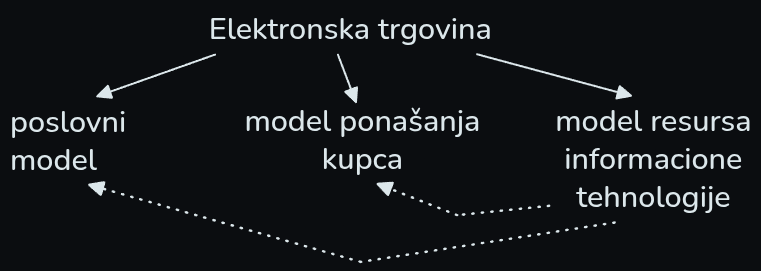
\includegraphics[width=0.6\textwidth]{slide2.png}
\end{figure}

\end{frame}

% =========================================================
% SLIDE 3
% =========================================================

\begin{frame}{Savremeni informacioni sistemi}

\metodologijaProblem{} Savremeni informacioni sistemi, uključujući sisteme elektronske trgovine, dominantno se zasnivaju na centralizovanom modelu u kojem se poverenje delegira trećim stranama sa kontrolom nad podacima i pravilima sistema.

To smanjuje autonomiju korisnika i stvara asimetriju moći, koja se ogleda u: \redColor{algoritamskoj kontroli}, \redColor{cenzuri i kontroli pristupa}, \redColor{koncentraciji moći}, \redColor{nadzornom kapitalizmu} i \redColor{zloupotrebi ličnih podataka}.

\metodologijaCilj{Analiza savremenih informacionih sistema elektronske trgovine, sa ciljem identifikacije njihovih ograničenja i implicitnih pretpostavki u pogledu poverenja i upravljanja podacima korisnika.}

\end{frame}

% =========================================================
% SLIDE 4
% =========================================================

\begin{frame}{Savremeni informacioni sistemi}

\vspace{-0.35cm}

\metodologijaProblem{} Uklanjanje centralizovanog autoriteta uvodi mogućnost neispravnog ili malicioznog ponašanja pojedinih učesnika, pri čemu sistem mora očuvati konzistentnost.

Decentralizacija zahteva \blueColor{otvoren sistem} bez \redColor{centralne kontrole} ili jedne tačke otkaza.

\metodologijaCilj{Uvođenje i formalizacija pojma decentralizacije kao proširenja klasične sociotehničke paradigme informacionih sistema.}

\vspace{-0.7cm}

\begin{figure}[ht]
\centering

\subfloat[Centralizovan]{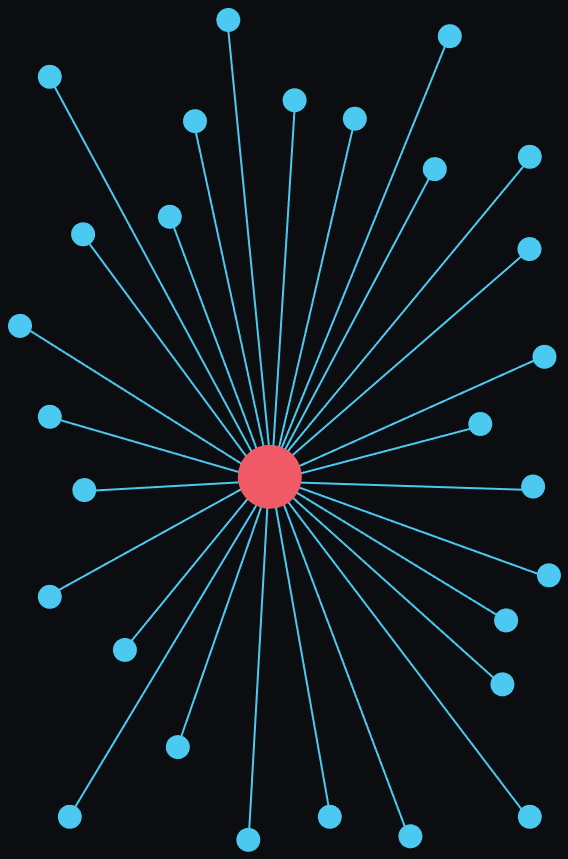
\includegraphics[width=0.19\textwidth]{slide4a.png}}
\hspace{1.2cm}
\subfloat[Distribuiran]{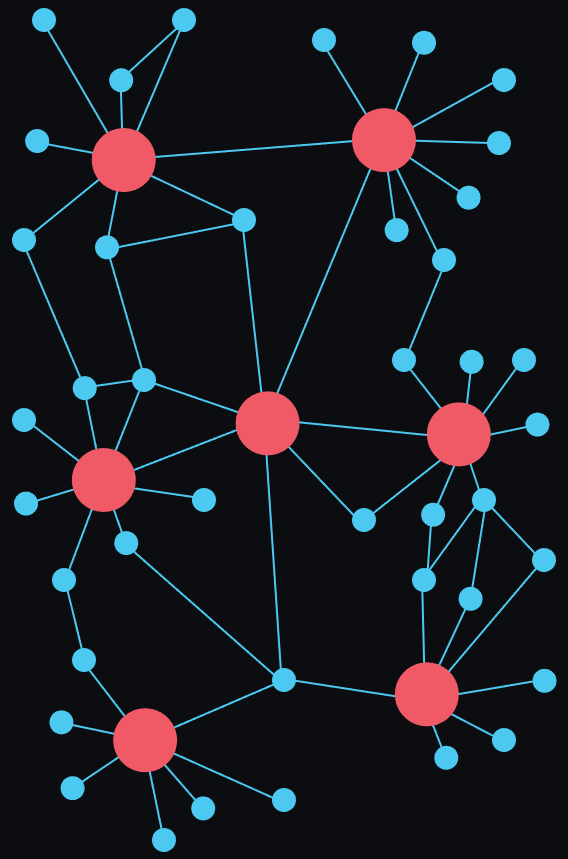
\includegraphics[width=0.19\textwidth]{slide4b.png}}
\hspace{1.2cm}
\subfloat[Decentralizovan]{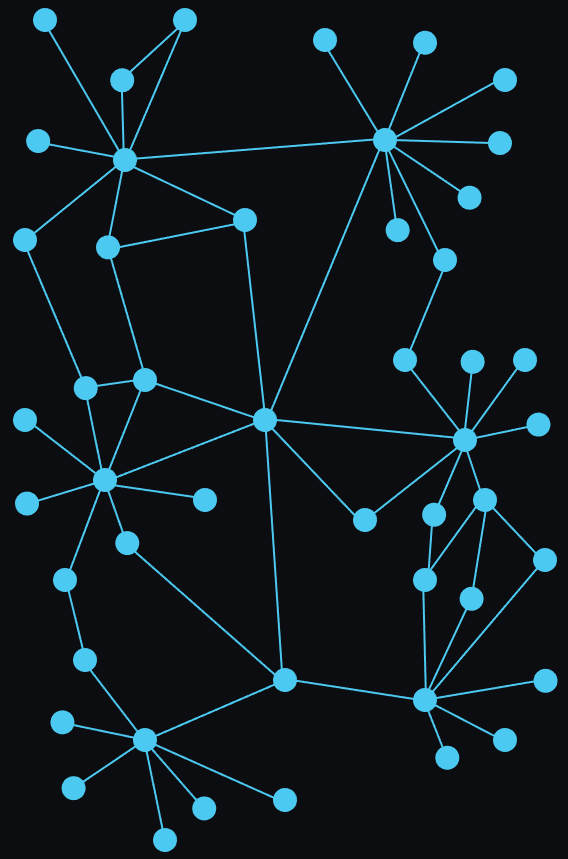
\includegraphics[width=0.19\textwidth]{slide4c.png}}

\caption{Arhitektonski modeli organizacije i upravljanja informacionim sistemima.}
\end{figure}

\end{frame}

% =========================================================
% SLIDE 5
% =========================================================

\begin{frame}{Savremeni informacioni sistemi}

Savremeni informacioni sistemi visokog kapaciteta proširuju kapacitet dodavanjem instanci i raspodelom opterećenja.

Iako je infrastrukturno distribuiran, sistem zadržava centralizovan model upravljanja kroz \redColor{klijent-server komunikaciju} zasnovanu na \redColor{lokacijskom adresiranju}.

Zato je potrebno uvesti model komunikacije zasnovan na \blueColor{mreži ravnopravnih čvorova} (\emph{peer-to-peer}), koji sistem čini otvorenim za učešće.

Koordinacija se ostvaruje algoritmima konsenzusa, među kojima su i deterministički BFT algoritmi zasnovani na razmeni poruka i glasanju između čvorova.

\metodologijaProblem{} Performanse opadaju sa porastom broja čvorova usled povećanja komunikacionog opterećenja.

\end{frame}

\end{document}

\end{document}